\documentclass[10pt,aspectratio=169]{beamer}

% https://de.overleaf.com/latex/templates/metropolis-beamer-theme/qzyvdhrntfmr
\usetheme[progressbar=frametitle]{metropolis}
\usepackage{appendixnumberbeamer}

\usepackage{booktabs}
\usepackage[scale=2]{ccicons}

\usepackage{pgfplots}
\usepgfplotslibrary{dateplot}

\usepackage{xspace}
\newcommand{\themename}{\textbf{\textsc{metropolis}}\xspace}

\usepackage{array}
\usepackage{ngerman}

\title{Eigengesichter}
\subtitle{Mentorierte Arbeit in Fachdidaktik Mathematik}
% \date{\today}
\date{}
\author{Oliver Rietmann}
\institute{ETH Zürich}
% \titlegraphic{\hfill\includegraphics[height=1.5cm]{logo.pdf}}

\begin{document}
	
\maketitle

%\section[Format und Ziele]{Format und Ziele}

\begin{frame}[fragile]{Form und Inhalt} 	
	\begin{columns}[T,onlytextwidth]
		\column{\textwidth}
		\metroset{block=fill}
		\begin{block}{Was?}
			Anleitung zur Implementierung eines Programms zur \textcolor{blue}{Gesichtserkennung} und \textcolor{blue}{Bildkomprimierung} in Python.
		\end{block}
		\vspace{0.2cm}
		\begin{block}{Wer?}
			Eine \textcolor{blue}{Schulklasse} oder eine einzelne Person.
		\end{block}
		\vspace{0.2cm}
		\begin{block}{Wie?}
			Anleitung als \textcolor{blue}{Fliesstext} mit Programmier- und Theorieaufgaben sowie Lösungen.
			Zudem werden \textcolor{blue}{Python Codes} zur Verfügung gestellt (Templates).
		\end{block}
	\end{columns}	
\end{frame}

\begin{frame}[fragile]{Eigengesichter}
	\begin{center}
		Bilder der Auflösung $\textcolor{blue}{M}\times\textcolor{green}{N}$ können als Vektoren in $\left[0,1\right]^{\textcolor{blue}{M}\cdot\textcolor{green}{N}}$ aufgefasst werden.
	\end{center}
	\begin{minipage}{0.45\textwidth}
		\begin{tabular}{m{2.0cm} m{0.5cm} c}
			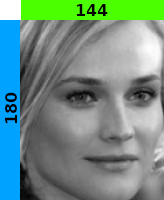
\includegraphics[width=0.3\textwidth]{images/vectormatrix/ImageToVector} &
			$\longrightarrow$ &
			$\begin{pmatrix}
				p_{1} \\
				p_{2} \\
				\vdots \\
				p_{\textcolor{blue}{M}\textcolor{green}{N}} \\
			\end{pmatrix}$ \\
			
\includegraphics[width=0.3\textwidth]{images/facespace/meanface} &
			$\longrightarrow$ &
			$\begin{pmatrix}
				m_{1} \\
				m_{2} \\
				\vdots \\
				m_{\textcolor{blue}{M}\textcolor{green}{N}} \\
			\end{pmatrix}$
		\end{tabular}
	\end{minipage}
	\begin{minipage}{0.45\textwidth}
		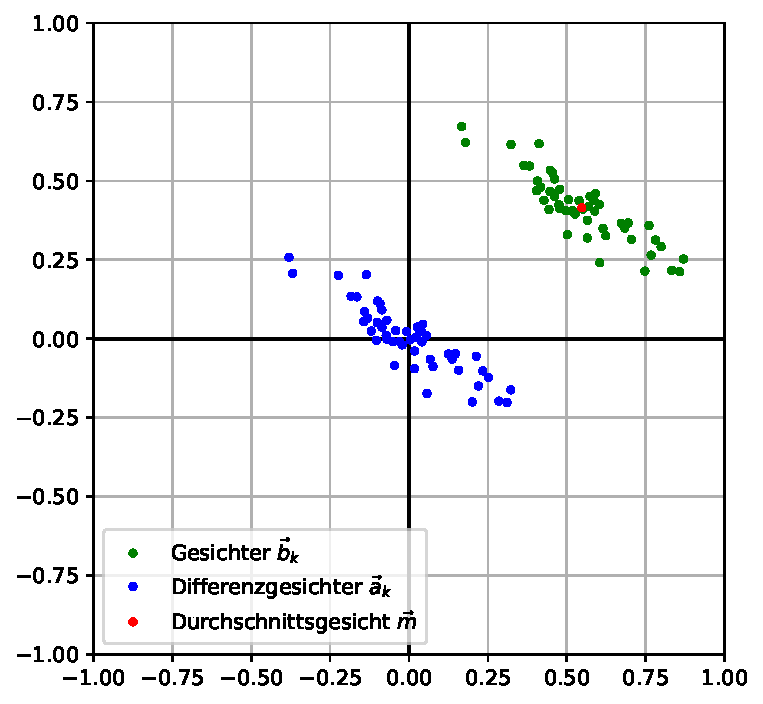
\includegraphics[width=\textwidth]{images/facespace/meandiff}
	\end{minipage}
\end{frame}

\begin{frame}[fragile]{Eigengesichter}
	\begin{center}
		Eine \textcolor{blue}{\textbf{Hauptkomponentenanalyse}} mittels \textcolor{blue}{\textbf{Singulärwertzerlegung}} liefert die \textcolor{blue}{\textbf{Eigengesichter}}.
	\end{center}
	\begin{tabular}{c}
		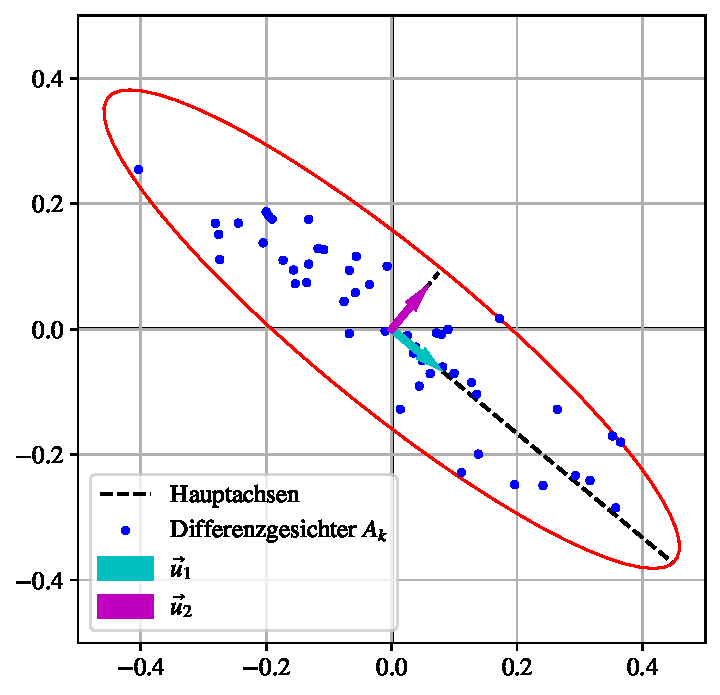
\includegraphics[width=0.45\textwidth]{images/facespace/principal_components}
	\end{tabular}
	\begin{tabular}{cccccccc}
		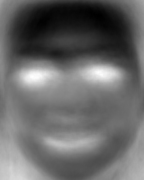
\includegraphics[width=0.095\textwidth]{images/eigenfaces/eigenface00} & 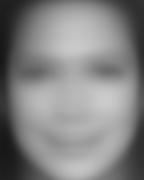
\includegraphics[width=0.095\textwidth]{images/eigenfaces/eigenface01} &
		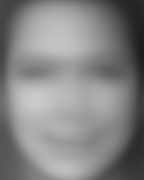
\includegraphics[width=0.095\textwidth]{images/eigenfaces/eigenface02} & 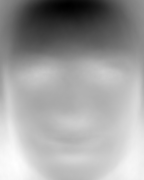
\includegraphics[width=0.095\textwidth]{images/eigenfaces/eigenface03} \\
		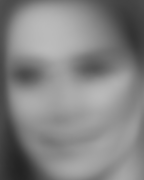
\includegraphics[width=0.095\textwidth]{images/eigenfaces/eigenface04} &
		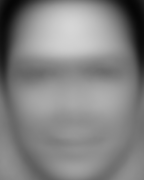
\includegraphics[width=0.095\textwidth]{images/eigenfaces/eigenface05} & 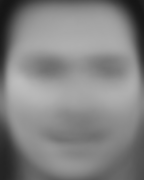
\includegraphics[width=0.095\textwidth]{images/eigenfaces/eigenface06} &
		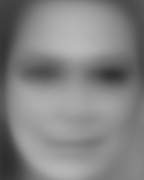
\includegraphics[width=0.095\textwidth]{images/eigenfaces/eigenface07} \\ 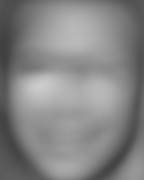
\includegraphics[width=0.095\textwidth]{images/eigenfaces/eigenface08} &
		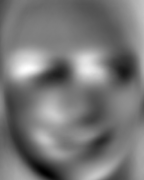
\includegraphics[width=0.095\textwidth]{images/eigenfaces/eigenface09} & 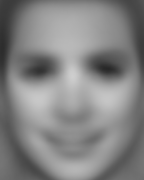
\includegraphics[width=0.095\textwidth]{images/eigenfaces/eigenface10} &
		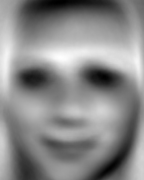
\includegraphics[width=0.095\textwidth]{images/eigenfaces/eigenface11}
	\end{tabular}
\end{frame}

\begin{frame}[fragile]{Konzeptwandel $\mathbb R^3\longrightarrow\mathbb R^{M\cdot N}$ (Projektion auf die Eigengesichter)}
	Gesichter als Überlagerung des Durchschnittsgesichtes und der Eigengeichter:\\[0.5cm]
	\begin{tabular}{m{1.3cm} c m{1.3cm} c m{1.3cm} c m{1.3cm} c m{1.3cm} c}
		$\quad\ \ \vec p$ & & $\quad\ \ \vec m$ & & $\quad\ \ \vec u_1$ & & $\quad\ \ \vec u_2$ & & $\quad\ \ \vec u_2$ & \\
		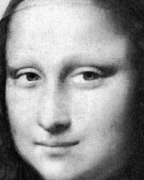
\includegraphics[width=0.1\textwidth]{images/eigenfaces/mona_lisa_eigen_approx} &
		$=$ & 
\includegraphics[width=0.1\textwidth]{images/facespace/meanface} & $+\ c_1$ & 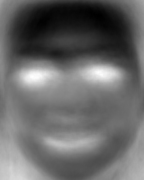
\includegraphics[width=0.1\textwidth]{images/eigenfaces/eigenface00}
		& $+\ c_2$ & 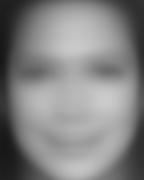
\includegraphics[width=0.1\textwidth]{images/eigenfaces/eigenface01} & $+\ c_3$ & 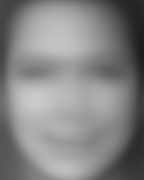
\includegraphics[width=0.1\textwidth]{images/eigenfaces/eigenface02} & $+\ \cdots$
	\end{tabular}\\[0.5cm]
	\begin{minipage}{0.45\textwidth}
		\begin{columns}[T,onlytextwidth]
			\column{\textwidth}
			\metroset{block=fill}
			\begin{block}{Aufbauen auf \textcolor{blue}{\textbf{Vorwissen}} im $\mathbb R^3$}
				\begin{itemize}
					\item Linearkombination
					\item Skalarprodukt
					\item Orthogonalität
				\end{itemize}
			\end{block}
		\end{columns}
	\end{minipage}\hfill
	\begin{minipage}{0.45\textwidth}
		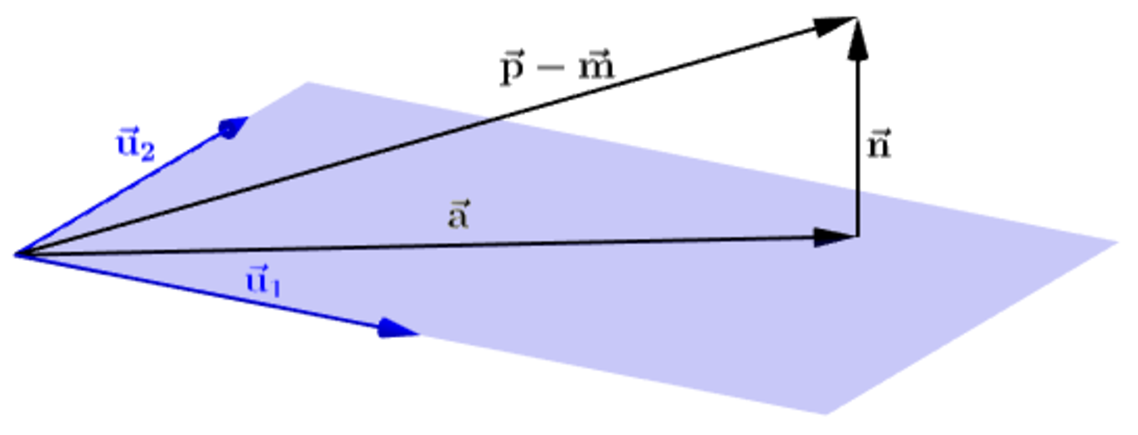
\includegraphics[width=\textwidth]{images/projection2}
	\end{minipage}
\end{frame}

\begin{frame}[fragile]{Problem-basiertes Lernen (Bildkompression)}
	\begin{minipage}{0.72\textwidth}
		\begin{columns}[T,onlytextwidth]
			\column{\textwidth}
			\metroset{block=fill}
			\begin{block}{Einstiegsfrage zur \textcolor{blue}{\textbf{kognitiven Aktivierung}}:}
				Absolutbeträge der Koeffizienten der Linearkombination bezüglich der \textcolor{blue}{\textbf{Differenzgesichter}} (links) und der \textcolor{blue}{\textbf{Eigengesichter}} (rechts).
				Was sind die Unterschiede und welche Bedeutung haben sie?
			\end{block}
		\end{columns}
	\end{minipage}\hfill
	\begin{minipage}{0.25\textwidth}
		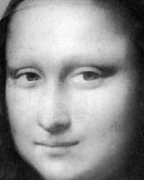
\includegraphics[width=0.45\textwidth]{images/eigenfaces/mona_lisa_naive_approx}
		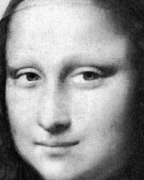
\includegraphics[width=0.45\textwidth]{images/eigenfaces/mona_lisa_eigen_approx}
	\end{minipage}
	\begin{tabular}{cc}
		\centering
		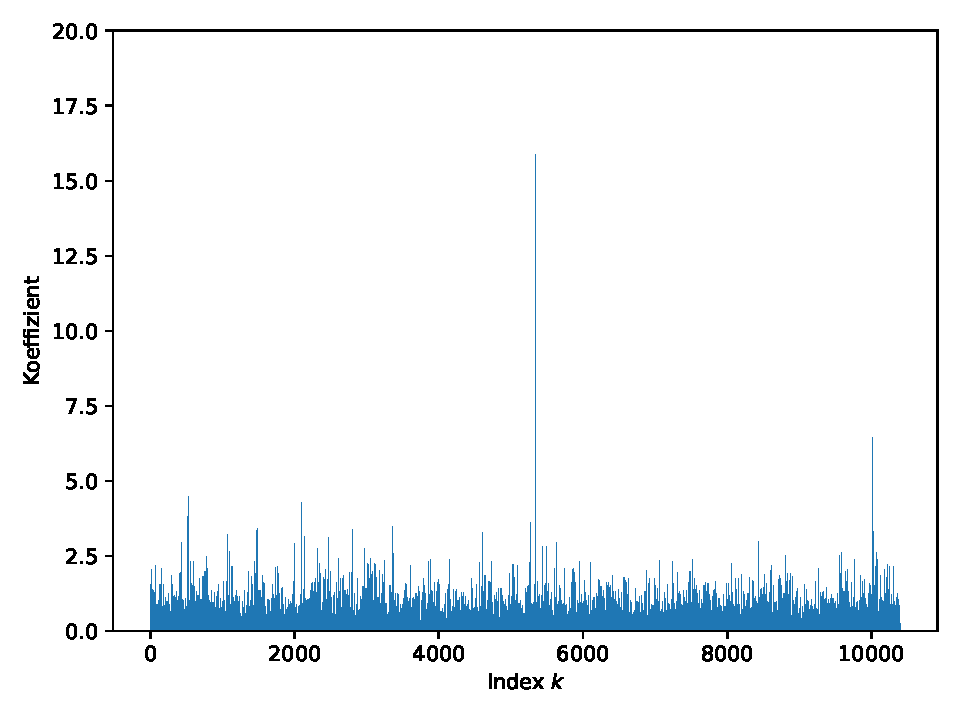
\includegraphics[width=0.45\textwidth]{images/eigenfaces/naive_coef} &
		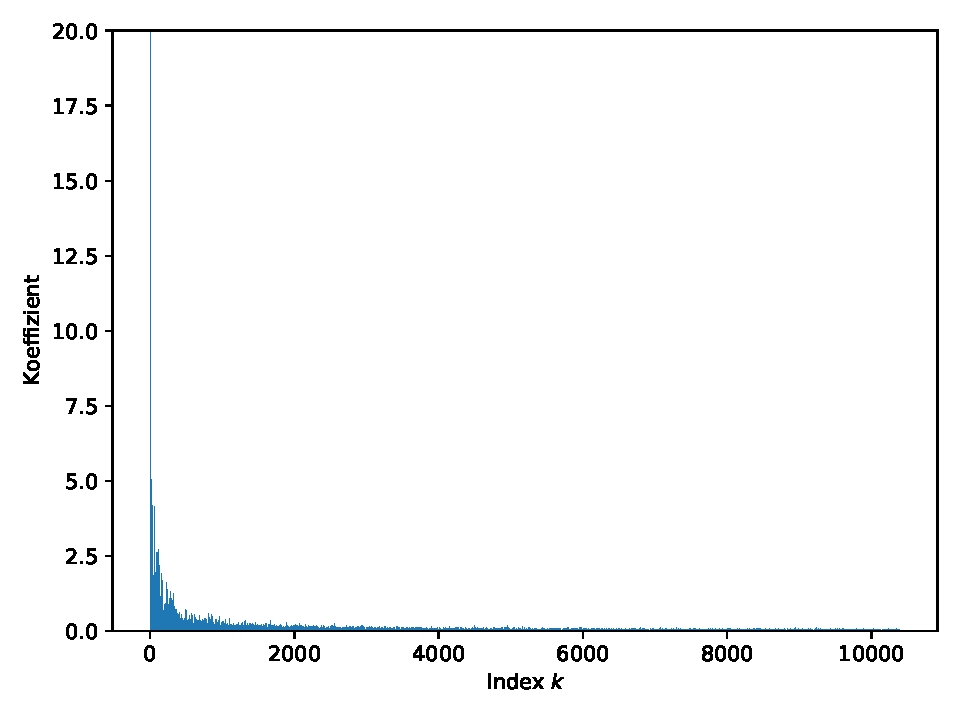
\includegraphics[width=0.45\textwidth]{images/eigenfaces/eigen_coef} \\
		\phantom{text}Differenzgesichter & \phantom{text}Eigengesichter
	\end{tabular}
\end{frame}

\begin{frame}[fragile]{Bildkompression}
	\begin{center}
	\begin{tabular}{cccc}
		$20$ & $200$ & $2000$ & Original \\
		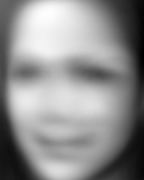
\includegraphics[width=0.1\textwidth]{images/compression/mona_lisa_20} &
		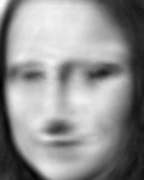
\includegraphics[width=0.1\textwidth]{images/compression/mona_lisa_200} &
		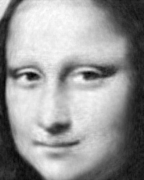
\includegraphics[width=0.1\textwidth]{images/compression/mona_lisa_2000} & 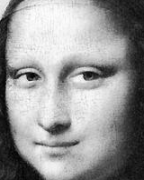
\includegraphics[width=0.1\textwidth]{images/compression/mona_lisa} \\
		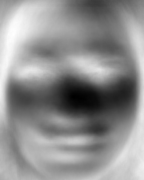
\includegraphics[width=0.1\textwidth]{images/compression/chair_20} &
		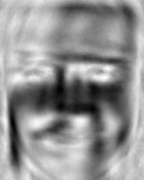
\includegraphics[width=0.1\textwidth]{images/compression/chair_200} &
		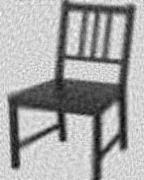
\includegraphics[width=0.1\textwidth]{images/compression/chair_2000} & 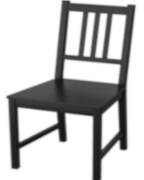
\includegraphics[width=0.1\textwidth]{images/compression/chair}
	\end{tabular}
	\end{center}
\end{frame}

\begin{frame}[fragile]{Zusammenfassung}
	Die Eigengesichter ...\\
	\vspace{0.5cm}
	\begin{enumerate}[1.] \setlength\itemsep{0.5cm}
		\item ... bauen auf der \textcolor{blue}{Vektorgeometrie im $\mathbb R^3$} auft.
		\item ... können Konzepte der linearen Algebra in höheren Dimensionen \textcolor{blue}{visualisieren}.
		\item ... können als \textcolor{blue}{Backbox} zur Verfügung gestellt werden.
		\item ... erlauben die Auseinandersetzung mit der \textcolor{blue}{linearen Algebra in höheren Dimensionen}.
	\end{enumerate}
\end{frame}

\begin{frame}[fragile]{Konzeptwandel $\mathbb R^3\longrightarrow\mathbb R^{M\cdot N}$ (Abstand Punkt-Gerade)}
	\begin{minipage}{0.45\textwidth}
		\begin{columns}[T,onlytextwidth]
			\column{\textwidth}
			\metroset{block=fill}
			\begin{block}{Abstand Punkt-Gerade im $\mathbb R^2$}
				\begin{itemize}
					\item Zeichnung (siehe rechts)
					\item konkrete Zahlen
				\end{itemize}
			\end{block}
			\begin{block}{Abstand Punkt-Gerade im $\mathbb R^4$}
				\begin{itemize}
					\item \textcolor{red}{keine Zeichnung möglich}
					\item konkrete Zahlen
				\end{itemize}
			\end{block}
			\begin{block}{Abstand Punkt-Gerade im $\mathbb R^{M\cdot N}$}
				\begin{itemize}
					\item \textcolor{red}{keine Zeichnung möglich}
					\item \textcolor{red}{keine Zahlen, nur Variablen}
				\end{itemize}
			\end{block}
		\end{columns}
	\end{minipage}\hfill
	\begin{minipage}{0.45\textwidth}
		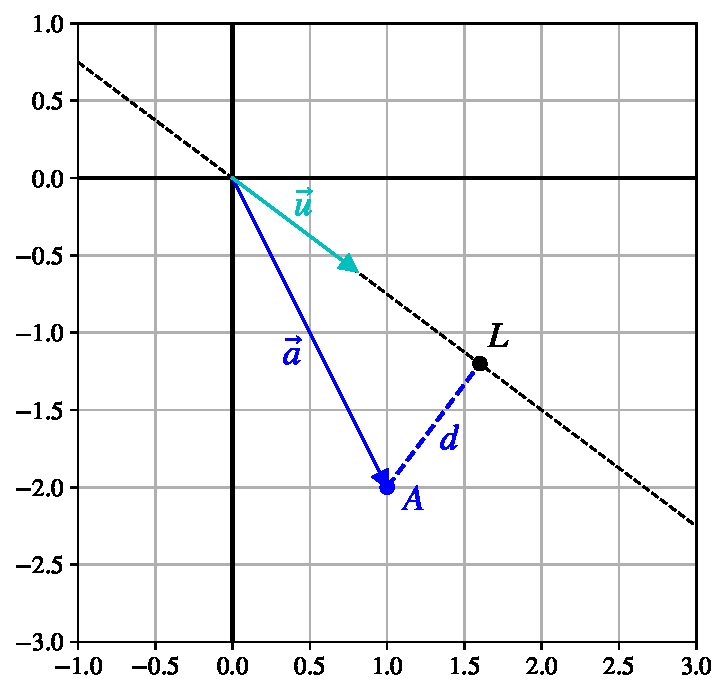
\includegraphics[width=\textwidth]{images/facespace/distance_simple}
	\end{minipage}
\end{frame}

\begin{frame}[fragile]{Gruppenarbeit (Erstellen der Datenbank)}
	\begin{columns}[T,onlytextwidth]
		\column{\textwidth}
		\metroset{block=fill}
		\begin{block}{Positive Interdependenz}
			Je mehr Bilder die Datenbank zu Verfügung hat, desto mächtiger werden die Anwendungen.
		\end{block}
		\begin{block}{Individuelle Verantwortlichkeit}
			Wenn jemand fehlerhafte Bilder beisteuert, wird das gesamte Programm nicht funktionieren.
		\end{block}
		\begin{block}{Förderliche Interaktionen}
			Erst wenn alle fertig sind, kann man abschliessen.
			Wer fertig ist, sollte den Anderen helfen.
		\end{block}
		\begin{block}{Kooperative Arbeitstechniken}
			Zusammenarbeit ist nur zwingend erforderlich, wenn die Bilder zusammengetragen werden.
		\end{block}
		\begin{block}{Reflexive Prozesse}
			Bilder zuschneiden hilft, ein Bild als eine $M\times N$ \glqq{}Matrix\grqq{} von Pixeln zu verstehen.
		\end{block}
	\end{columns}
\end{frame}

\begin{frame}[fragile]{Selbsterklärung (Bilder als Vektoren)}
	\begin{minipage}{0.6\textwidth}
		\begin{columns}[T,onlytextwidth]
			\column{\textwidth}
			\metroset{block=fill}
			\begin{block}{Aufgabe}
				Nennen Sie einen Unterschied und eine Gemeinsamkeit der vereinfachten Darstellung rechts zu unserer Situation (Auflösung $M=180$ und $N=144$).
			\end{block}
			\begin{block}{Aufgabe}
				Kann man die Differenzgesichter wieder als Bilder darstellen?
			\end{block}
		\end{columns}
	\end{minipage}\hfill
	\begin{minipage}{0.35\textwidth}
		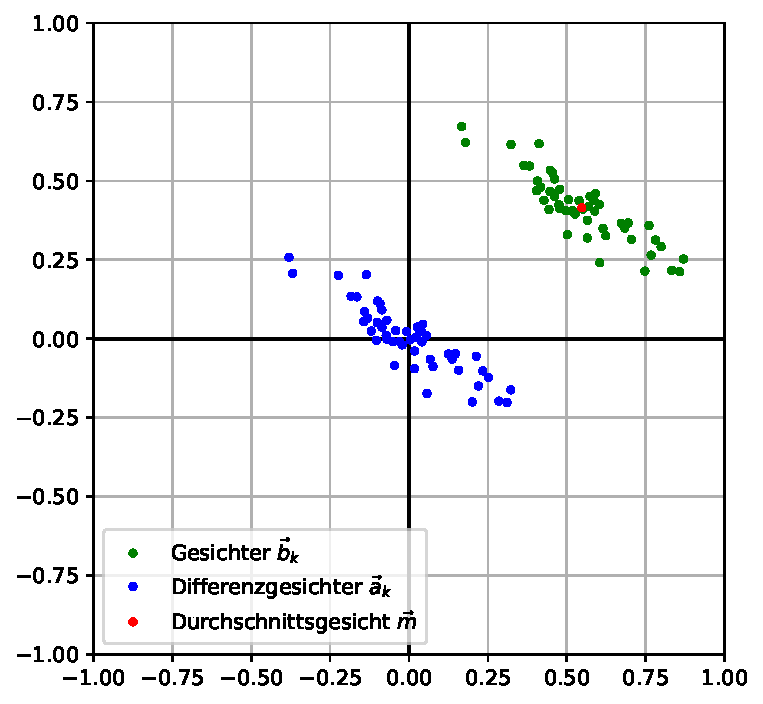
\includegraphics[width=\textwidth]{images/facespace/meandiff}
	\end{minipage}
\end{frame}

\begin{frame}[fragile]{Weitere Didaktische Aspekte}
	\begin{columns}[T,onlytextwidth]
		\column{\textwidth}
		\metroset{block=fill}
		\begin{block}{Scaffolding}
			\begin{itemize}
				\item Berechnung der Eigengesichter mit SVD zu schwierig $\rightarrow$ \textcolor{blue}{Eigengesichter als Blackbox}.
				\item Einlesen/Abspeichern von Bildern hat nichts mit Mathematik zu tun $\rightarrow$ \textcolor{blue}{Code-Templates}.
			\end{itemize}
		\end{block}
		\begin{block}{Interleaved practive}
			\begin{itemize}
				\item \textcolor{blue}{blocked}: Zuerst ganze Theorie herleiten, dann nur noch programmieren
				\item \textcolor{blue}{interleaved}: Abwechslungsweise Theorie und programmieren.
			\end{itemize}
		\end{block}
		\begin{block}{Holistic mental model confrontation}
			Verlgleiche vereinfachte Darstellungen in \textcolor{blue}{3} Dimensionen mit \textcolor{blue}{$N\cdot M$} Dimensionen.
		\end{block}
	\end{columns}
\end{frame}
	
\end{document}